\section{Bonus}
This section uses the variance Criterion to find the $\pi$ number. Here is the result of the $\pi$ estimation with different variances:
\begin{itemize}
    \item $\sigma = 10^{-4}$
    \begin{figure}[H] 
     	\caption{$\sigma = 10^{-4}$ result} 
     	\centering 
     	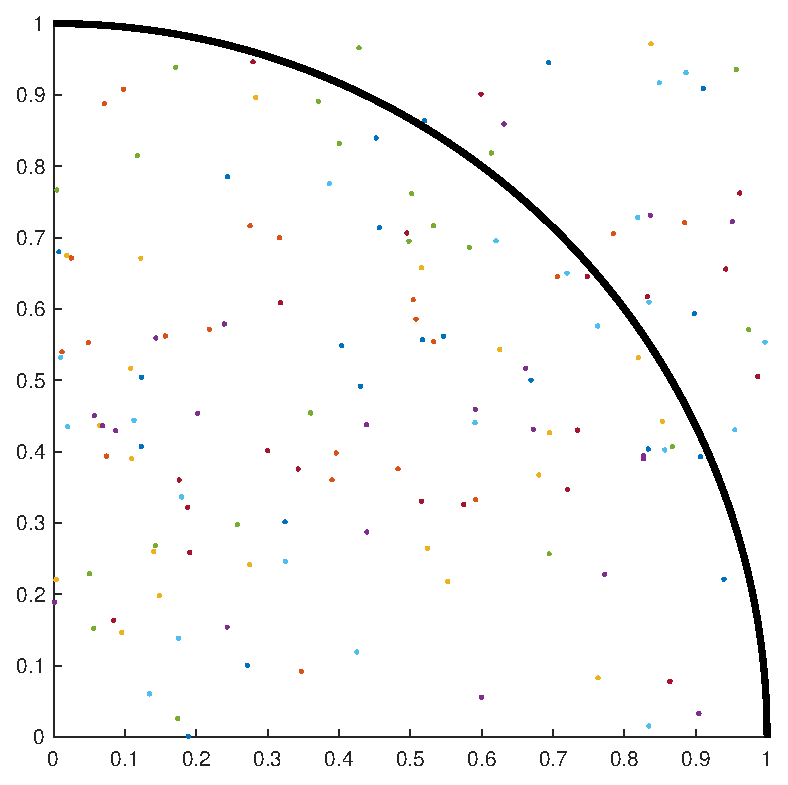
\includegraphics[width=12cm]{../Figure/Bonus/mont_e4} 
    \end{figure}
    \item $\sigma = 10^{-5}$
    \begin{figure}[H] 
        \caption{$\sigma = 10^{-5}$ result} 
        \centering 
        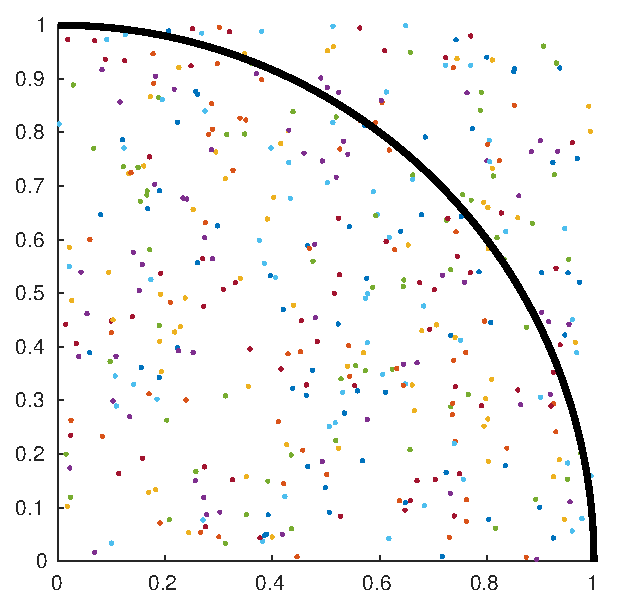
\includegraphics[width=12cm]{../Figure/Bonus/mont1e-05.eps} 
   \end{figure}
    \item $\sigma = 10^{-6}$
    \begin{figure}[H] 
        \caption{$\sigma = 10^{-6}$ result} 
        \centering 
        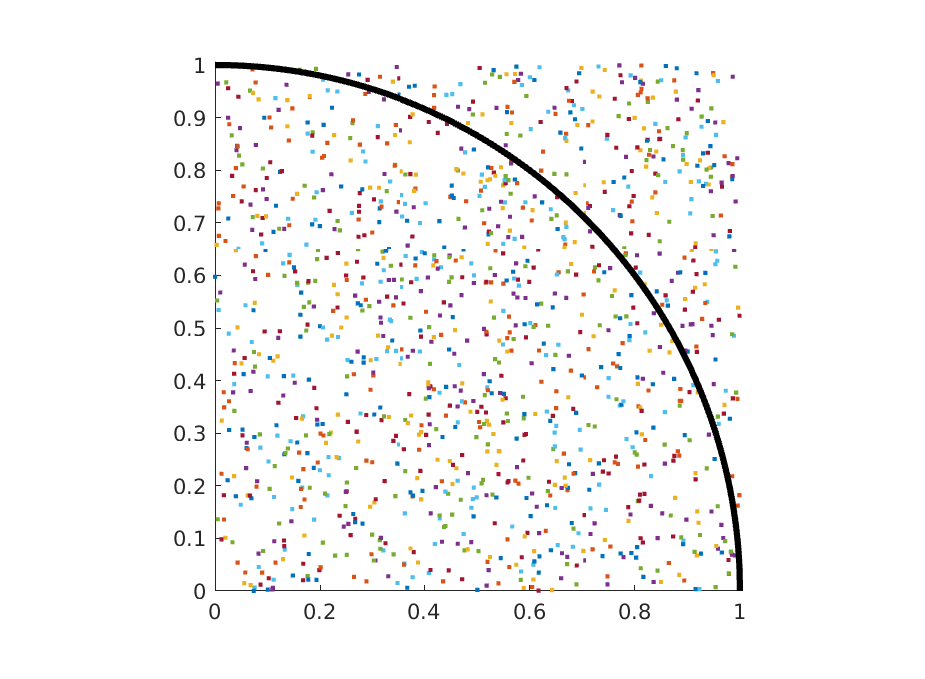
\includegraphics[width=12cm]{../Figure/Bonus/mont1e-06.eps} 
   \end{figure}
    \item $\sigma = 10^{-7}$
    \begin{figure}[H] 
        \caption{$\sigma = 10^{-7}$ result} 
        \centering 
        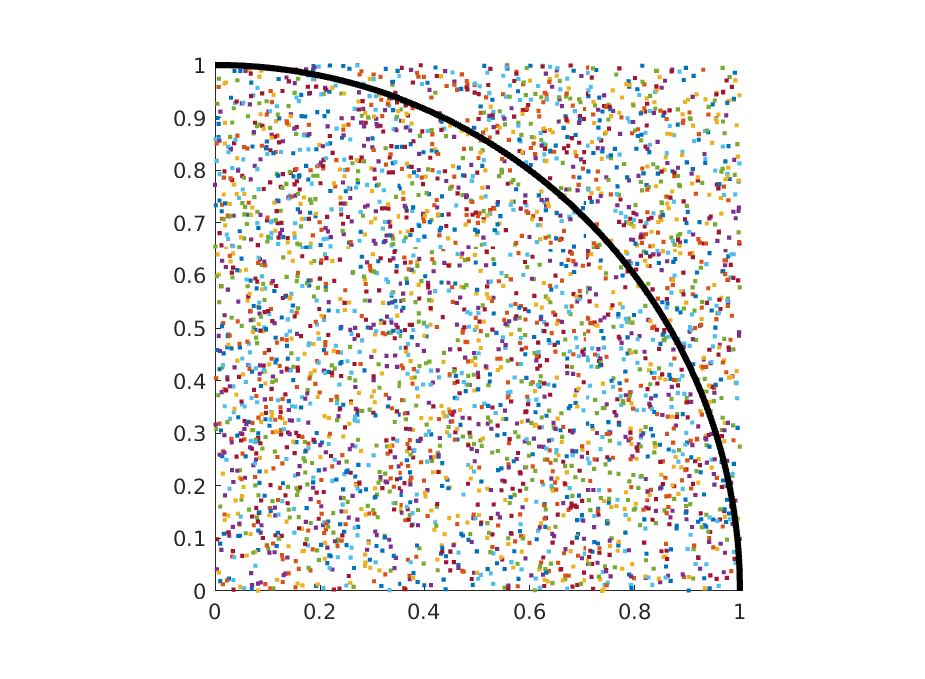
\includegraphics[width=12cm]{../Figure/Bonus/mont1e-07.eps} 
   \end{figure}
    \item $\sigma = 10^{-8}$
    \begin{figure}[H] 
        \caption{$\sigma = 10^{-8}$ result} 
        \centering 
        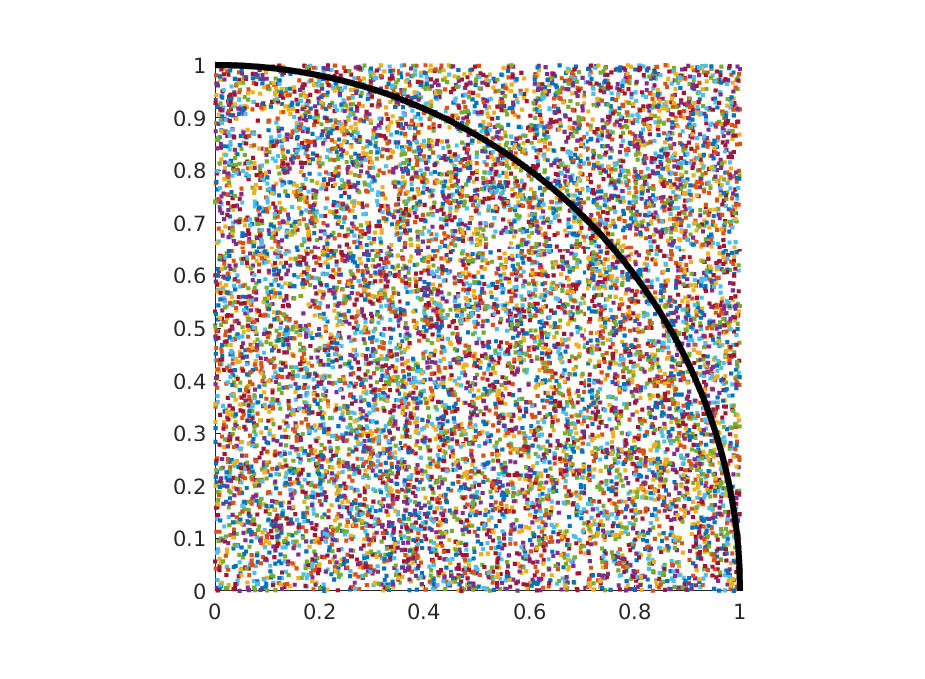
\includegraphics[width=12cm]{../Figure/Bonus/mont1e-08.eps} 
   \end{figure}
    \item $\sigma = 10^{-9}$
    \begin{figure}[H] 
        \caption{$\sigma = 10^{-9}$ result} 
        \centering 
        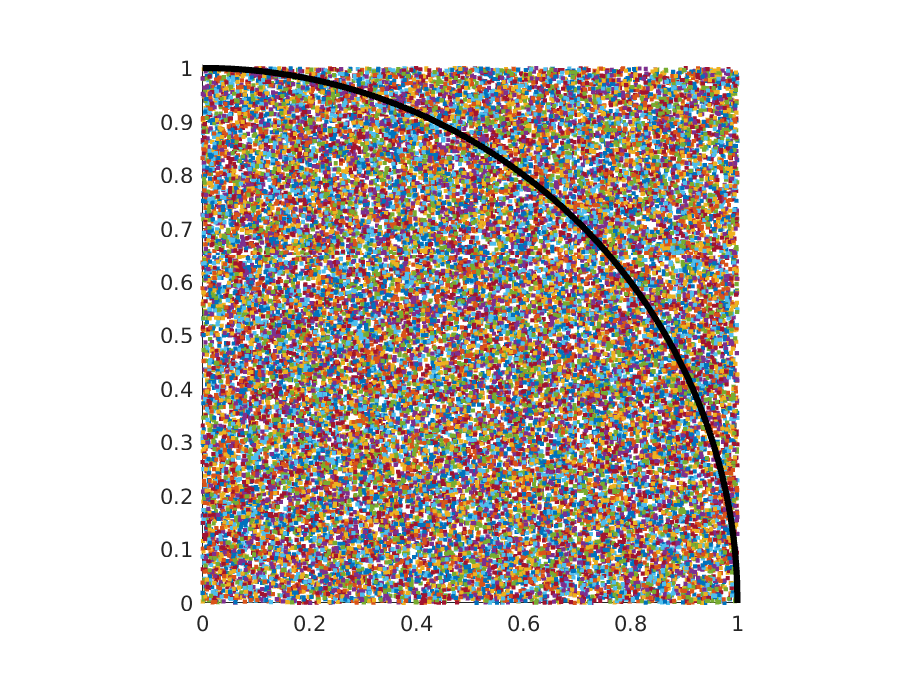
\includegraphics[width=12cm]{../Figure/Bonus/mont1e-09.eps} 
   \end{figure}
\end{itemize}